% ============================================================
% Figure 4: OPD Failure Progression (3-panel, full width)
% ============================================================
\begin{figure*}[t]
\centering
\begin{subfigure}[b]{0.33\textwidth}
\centering
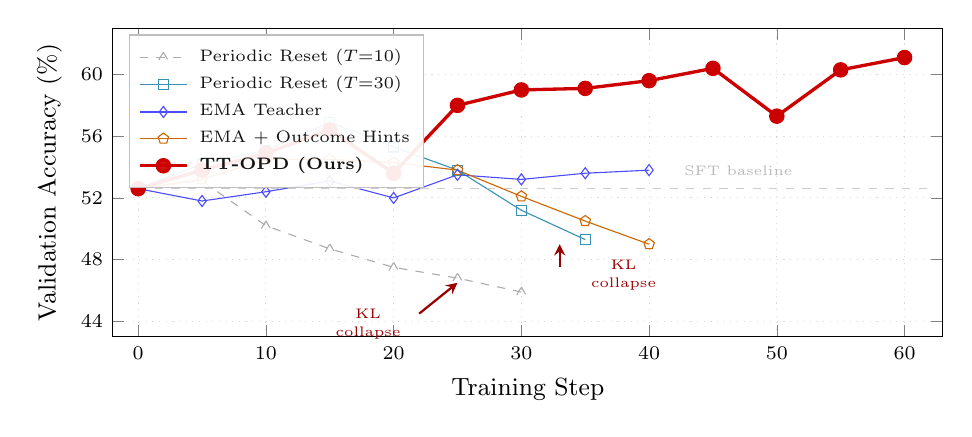
\begin{tikzpicture}
\begin{axis}[
    width=\textwidth,
    height=5.5cm,
    xlabel={Training Step},
    ylabel={Validation Accuracy (\%)},
    xmin=-2, xmax=63,
    ymin=43, ymax=63,
    xtick={0,10,20,30,40,50,60},
    ytick={44,48,52,56,60},
    grid=major,
    grid style={dotted, gray!30},
    tick label style={font=\scriptsize},
    label style={font=\small},
    legend style={at={(0.02,0.98)}, anchor=north west, font=\fontsize{6}{7.5}\selectfont, row sep=0pt, column sep=2pt, draw=gray!50, fill=white, fill opacity=0.92, inner sep=3pt},
    legend cell align={left},
    clip=false,
]
% Periodic Reset (short interval)
\addplot[color=gray!65, mark=triangle, mark size=1.8pt, thin, dashed] coordinates {
    (0,52.6) (5,53.1) (10,50.2) (15,48.7) (20,47.5) (25,46.8) (30,45.9)
};
\addlegendentry{Periodic Reset ($T{=}10$)}

% Periodic Reset (long interval)
\addplot[color=cyan!70!black, mark=square, mark size=1.8pt, thin] coordinates {
    (0,52.6) (5,54.2) (10,55.1) (15,56.9) (20,55.3) (25,53.8) (30,51.2) (35,49.3)
};
\addlegendentry{Periodic Reset ($T{=}30$)}

% EMA Teacher (no conditioning)
\addplot[color=blue!70, mark=diamond, mark size=2pt, thin] coordinates {
    (0,52.6) (5,51.8) (10,52.4) (15,53.1) (20,52.0) (25,53.5) (30,53.2) (35,53.6) (40,53.8)
};
\addlegendentry{EMA Teacher}

% EMA + Outcome Hints
\addplot[color=orange!80!black, mark=pentagon, mark size=2pt, thin] coordinates {
    (0,52.6) (5,53.2) (10,54.5) (15,54.5) (20,54.3) (25,53.8) (30,52.1) (35,50.5) (40,49.0)
};
\addlegendentry{EMA + Outcome Hints}

% Full TT-OPD (ours) -- BOLD RED
\addplot[color=red!80!black, mark=*, mark size=2.2pt, very thick] coordinates {
    (0,52.6) (5,53.8) (10,54.9) (15,56.4) (20,53.6) (25,58.0) (30,59.0) (35,59.1) (40,59.6) (45,60.4) (50,57.3) (55,60.3) (60,61.1)
};
\addlegendentry{\textbf{TT-OPD (Ours)}}

% Baseline reference
\addplot[dashed, gray!40, very thin] coordinates {(0,52.6) (62,52.6)};
\node[font=\fontsize{5.5}{6.5}\selectfont, gray!55, anchor=south west] at (axis cs:42,52.8) {SFT baseline};

% KL collapse annotation on Periodic Reset (T=10)
\draw[->, >=stealth, red!60!black, thick] (axis cs:22,44.5) -- (axis cs:25,46.5);
\node[font=\fontsize{5.5}{6.5}\selectfont, red!60!black, align=center] at (axis cs:18,43.8) {KL\\collapse};

% KL collapse annotation on Periodic Reset (T=30)
\draw[->, >=stealth, red!60!black, thick] (axis cs:33,47.5) -- (axis cs:33,49.0);
\node[font=\fontsize{5.5}{6.5}\selectfont, red!60!black, align=center] at (axis cs:38,47.0) {KL\\collapse};

\end{axis}
\end{tikzpicture}
\caption{Validation Accuracy}
\label{fig:opd_acc}
\end{subfigure}%
\hfill
\begin{subfigure}[b]{0.33\textwidth}
\centering
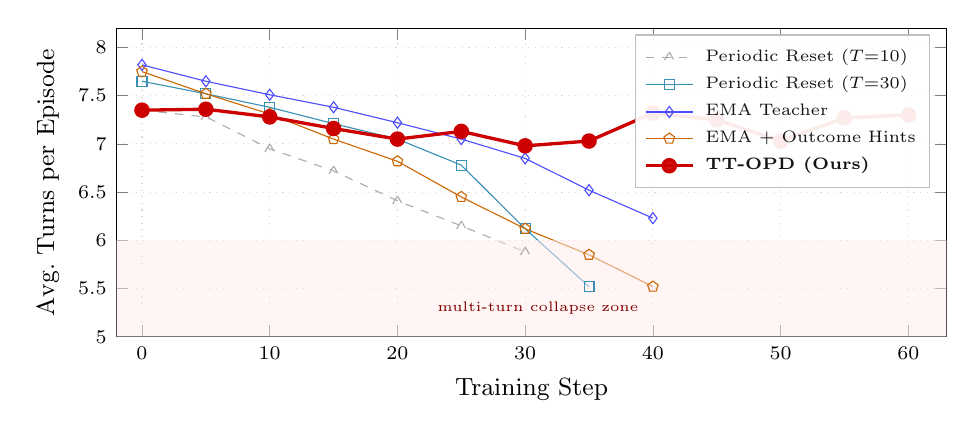
\begin{tikzpicture}
\begin{axis}[
    width=\textwidth,
    height=5.5cm,
    xlabel={Training Step},
    ylabel={Avg.\ Turns per Episode},
    xmin=-2, xmax=63,
    ymin=5.0, ymax=8.2,
    xtick={0,10,20,30,40,50,60},
    ytick={5.0,5.5,6.0,6.5,7.0,7.5,8.0},
    grid=major,
    grid style={dotted, gray!30},
    tick label style={font=\scriptsize},
    label style={font=\small},
    legend style={at={(0.98,0.98)}, anchor=north east, font=\fontsize{6}{7.5}\selectfont, row sep=0pt, column sep=2pt, draw=gray!50, fill=white, fill opacity=0.92, inner sep=3pt},
    legend cell align={left},
]
% Periodic Reset (short interval)
\addplot[color=gray!65, mark=triangle, mark size=1.8pt, thin, dashed] coordinates {
    (0,7.35) (5,7.28) (10,6.95) (15,6.72) (20,6.41) (25,6.15) (30,5.88)
};
\addlegendentry{Periodic Reset ($T{=}10$)}

% Periodic Reset (long interval)
\addplot[color=cyan!70!black, mark=square, mark size=1.8pt, thin] coordinates {
    (0,7.65) (5,7.52) (10,7.38) (15,7.21) (20,7.05) (25,6.78) (30,6.12) (35,5.52)
};
\addlegendentry{Periodic Reset ($T{=}30$)}

% EMA Teacher
\addplot[color=blue!70, mark=diamond, mark size=2pt, thin] coordinates {
    (0,7.82) (5,7.65) (10,7.51) (15,7.38) (20,7.22) (25,7.05) (30,6.85) (35,6.52) (40,6.23)
};
\addlegendentry{EMA Teacher}

% EMA + Outcome Hints
\addplot[color=orange!80!black, mark=pentagon, mark size=2pt, thin] coordinates {
    (0,7.75) (5,7.52) (10,7.31) (15,7.05) (20,6.82) (25,6.45) (30,6.12) (35,5.85) (40,5.52)
};
\addlegendentry{EMA + Outcome Hints}

% Full TT-OPD -- BOLD RED
\addplot[color=red!80!black, mark=*, mark size=2.2pt, very thick] coordinates {
    (0,7.35) (5,7.36) (10,7.28) (15,7.16) (20,7.05) (25,7.13) (30,6.98) (35,7.03) (40,7.32) (45,7.25) (50,7.03) (55,7.27) (60,7.30)
};
\addlegendentry{\textbf{TT-OPD (Ours)}}

% Multi-turn collapse zone
\fill[red!8, opacity=0.5] (axis cs:-2,5.0) rectangle (axis cs:63,6.0);
\node[font=\fontsize{5.5}{6.5}\selectfont, red!50!black] at (axis cs:31,5.3) {multi-turn collapse zone};

\end{axis}
\end{tikzpicture}
\caption{Average Turns per Episode}
\label{fig:opd_turns}
\end{subfigure}%
\hfill
\begin{subfigure}[b]{0.33\textwidth}
\centering
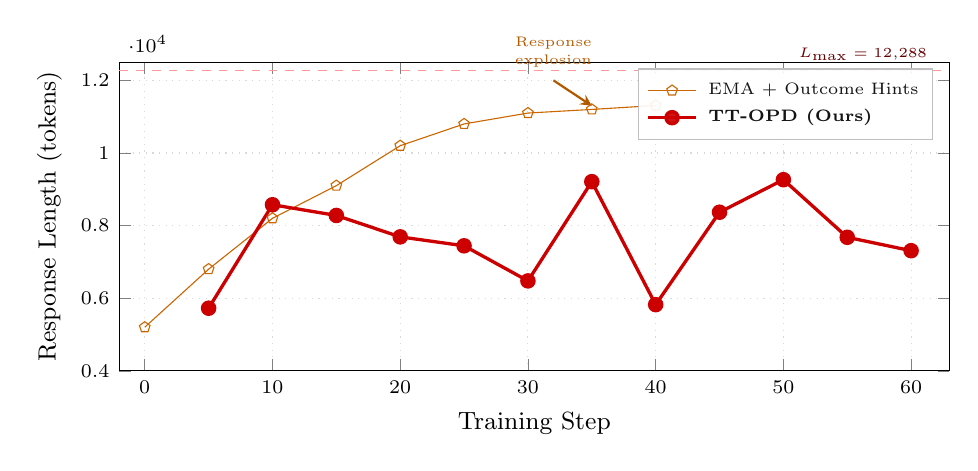
\begin{tikzpicture}
\begin{axis}[
    width=\textwidth,
    height=5.5cm,
    xlabel={Training Step},
    ylabel={Response Length (tokens)},
    xmin=-2, xmax=63,
    ymin=4000, ymax=12500,
    xtick={0,10,20,30,40,50,60},
    ytick={4000,6000,8000,10000,12000},
    yticklabel style={/pgf/number format/fixed, /pgf/number format/1000 sep={\,}},
    grid=major,
    grid style={dotted, gray!30},
    tick label style={font=\scriptsize},
    label style={font=\small},
    legend style={at={(0.98,0.98)}, anchor=north east, font=\fontsize{6}{7.5}\selectfont, row sep=0pt, column sep=2pt, draw=gray!50, fill=white, fill opacity=0.92, inner sep=3pt},
    legend cell align={left},
    clip=false,
]
% EMA + Outcome Hints -- shows response explosion
\addplot[color=orange!80!black, mark=pentagon, mark size=2pt, thin] coordinates {
    (0,5200) (5,6800) (10,8200) (15,9100) (20,10200) (25,10800) (30,11100) (35,11200) (40,11308)
};
\addlegendentry{EMA + Outcome Hints}

% Full TT-OPD -- controlled length
\addplot[color=red!80!black, mark=*, mark size=2.2pt, very thick] coordinates {
    (5,5724) (10,8574) (15,8279) (20,7689) (25,7443) (30,6476) (35,9210) (40,5822) (45,8368) (50,9264) (55,7677) (60,7308)
};
\addlegendentry{\textbf{TT-OPD (Ours)}}

% L_max line
\addplot[dashed, red!40, very thin] coordinates {(-2,12288) (63,12288)};
\node[font=\fontsize{5.5}{6.5}\selectfont, red!40!black, anchor=south east] at (axis cs:62,12288) {$L_{\max}=12{,}288$};

% Response explosion annotation
\draw[->, >=stealth, orange!70!black, thick] (axis cs:32,12000) -- (axis cs:35,11300);
\node[font=\fontsize{5.5}{6.5}\selectfont, orange!70!black, align=center, anchor=south] at (axis cs:32,12100) {Response\\explosion};

\end{axis}
\end{tikzpicture}
\caption{Response Length (tokens)}
\label{fig:opd_resplen}
\end{subfigure}
\caption{Ablation of distillation components across training. Each curve adds one component to isolate its effect. (a)~\textbf{Validation accuracy}: periodic teacher resets (both $T{=}10$ and $T{=}30$) suffer KL collapse---the distillation gradient is destroyed when the teacher is abruptly overwritten with student weights. EMA teacher alone plateaus near the baseline without outcome-aware signal. Adding outcome hints initially improves accuracy but collapses without length control. Only TT-OPD sustains improvement to 61.1\%. (b)~\textbf{Average turns}: all ablation variants decline monotonically toward single-turn behavior ($<$6 turns), while TT-OPD maintains 7.0--7.4 turns throughout training. (c)~\textbf{Response length}: without cosine length reward, outcome hints cause unchecked response growth toward $L_{\max}$; TT-OPD keeps responses bounded between 5.7K and 9.3K tokens.}
\label{fig:opd_failure}
\end{figure*}

